%
%   Chapter Introduction
%
%   author: Qing-Cheng Li r01922024 at csie dot ntu dot edu dot tw
%
\chapter{緒論}
\label{c:intro}

近年來,隨著網際網路的快速發展,網際網路中開始出現越來越多彙整人類知識的網站與資源,
如Wikipedia\footnote{http://www.wikipedia.org/},目前已經有超過280種語言,其中光是英語的條目就超過4,500,000條,
是透過來自世界各地的志願編輯者一字一句的貢獻建立而成的。

除了讓世界各地的人們可以在網際網路上共享知識之外,也讓計算機得以利用人類的知識,
輔助、改善、甚至自動化人工智慧、資料探勘與擷取、知識汲取、自動問答系統等任務,

為了達成此一目的,讓計算機可以看懂人類的知識,於是,
便出現了各式各樣透過擷取人工建立的知識資源,產生的結構化知識資料庫,並彼此相互鏈結。
如圖\ref{i:lod}所示,目前已有不少的結構化知識庫。
這些各式各樣的資源的最源頭,還是透過人類一字一句編輯產生的。% FIXME

\begin{figure}
\centering
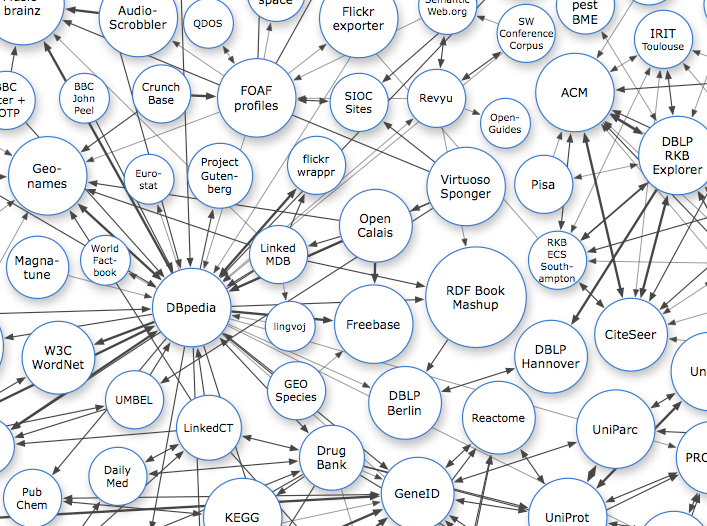
\includegraphics[width=0.5\textwidth]{images/01-lod-datasets}
\caption{各種結構化知識資料庫之間的鏈結}
\label{i:lod}
資料來源:linkeddata.org(2011)
\end{figure}

%
%   Background
%
\section{背景介紹}
在現今這個資訊社會,每當有新的事件發生時,例如某人的出生或死亡、某政治人物贏得了選舉、某地發生了天災等等,
這些資訊便會在網路上透過網路新聞、網誌、論壇、社群網站、微網誌等管道流傳。
新事件的發生代表了一些舊有的知識可能需要更新,例如修改某個人物的生死狀態、某個政治人物的勝選記錄等,
如有Wikipedia的志願編輯者注意到這些資訊之後,便會據此更新Wikipedia上關於某人或某球隊的條目。

如Wikipedia這種用來記錄實體(Entity)、實體的特性(Properties)、實體與實體間的關係(Relationships)的資料庫被稱為知識庫(Knowledge Base)。
以Wikipedia來說,Wikipedia以文章的形式儲存了人物、組織、公司、城市、事件等實體,
並在文章的文句中以超連結(Hyperlink)的形式描述實體與實體間的關係。
而文章中的資訊框(Infoboxes)則以半結構化的形式描述了實體的特性,如圖\ref{i:wiki}。

\begin{figure}
\centering
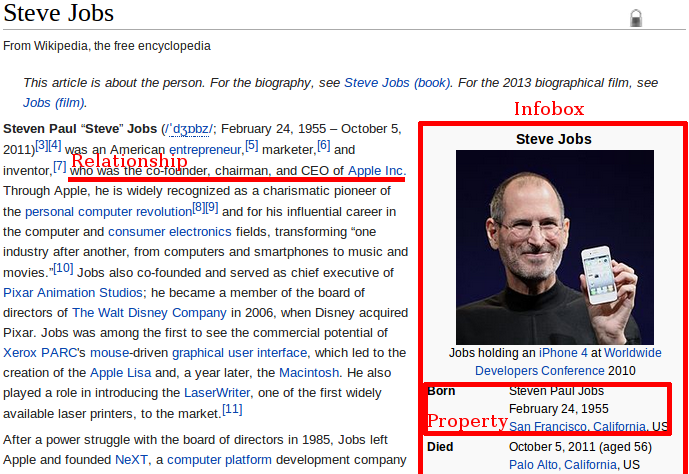
\includegraphics[width=0.65\textwidth]{images/01-wiki-as-kb}
\caption{Wikipedia中的文章}
\label{i:wiki}
\end{figure}

除了Wikipedia之外,還有其他DBpedia\cite{dbpedia-swj}、YAGO\cite{suchanek2007WWW}、Freebase\cite{freebase}等規模大小不一、不同應用的知識庫。
其中YAGO、DBpedia是透過自動化的方法擷取Wikipedia的內容,Freebase仰賴社群更新,這些知識庫都直接或間接仰賴人力更新。  %FIXME

%
%   Motivation
%
\section{研究動機}
% 知識庫不會憑空產生,多半是擷取人工編輯的成果或靠人工編輯,因此如何讓人工編輯的速度可以跟上知識產生的速度便成為一個重要的課題。
% TODO
% Keyword: 知識庫加速
知識庫仰賴志願編輯者的維護與更新,但這些人數比起資料庫中記錄的實體顯然非常的少。
這意味著知識庫的更新總是落後於新知識(過去從來不知道的知識與舊有知識內容的更動)的產生,
當新知識產生一段時日之後,知識庫的維護者才會更新知識庫,
圖\ref{i:wikicitenews}\cite{kba2012}表現了這種落後可能達一年甚至更長。
因此,如何讓人工編輯的速度可以跟上新知識出現的速度便成為一個重要的課題。

\begin{figure}
    \centering
    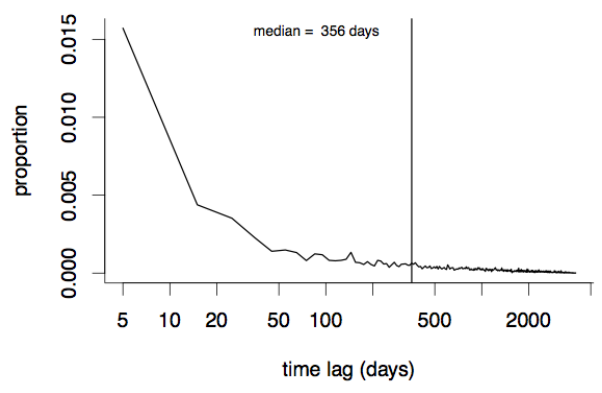
\includegraphics[width=0.5\textwidth]{images/01-wiki-cite-delay}
    \caption{Time lag for a sample of ~60,000 web pages cited by WP articles}
    \label{i:wikicitenews}
\end{figure}

為了縮短這個差距,自2012年起至今的每年美國NIST\footnote{National Institue of Standards and Technology}的TREC\footnote{Text Retriveal Conference}都會舉辦知識庫加速(Knowledge Base Acceleration, KBA)競賽,
希望參賽者可以建立一個系統,從由新聞、部落格、論壇等內容所組成、依時間所排列的龐大內容串流\footnote{2012年包含了4,973個小時,2013年包含了11,948小時。每小時包含約100,000份文件。}(Content Strean)中,
對有興趣的實體\footnote{2012年有27個人物、2個組織,2013年有98個人物,12個組織與24個設施。},包含了人物、組織或建築,進行過濾,
推薦文件給知識庫的編輯者,建議編輯者這份文件可能含有新的知識可供更新知識庫。

要從可能包含新知識的內容串流中,過濾出可能可以協助更新知識庫的文件,
則需要知道文章中是否包含知識。知識庫中實體間的關係、實體的特性就是一種知識,
我們想要知道一份來自內容串流的文件是否提及實體的特性,
例如句子「Jobs was born in San Francisco, California on February 24, 1955」中就包含了實體Jobs及其出生地這項特性的知識。
如果可以知道文章中是否包含這些資訊,便能夠進一步地協助知識庫的更新與維護。

% TODO
% We want to fill the Knowledge gap, do it fast

%
%   Goal
%
\section{研究目標}
% Keyword: given a content stream, 回答有沒有某個特性這樣
% TODO

%
%   Structure
%
\section{論文架構}  % TODO FIXME
本論文共分成五個章節。
第一章是緒論,簡介本研究的背景、動機與目標。
第二章是文獻探討,列舉了一些相關的研究與資源。
第三章是研究方法,提出如何於內容串流中究偵測實體特性的方法與步驟。
第四章是實驗結果與分析,
第五章是結論與未來展望,

